\section{Background and related work}
\label{sec:background}

\subsection{Stochastic rounding}

Let a binary floating-point format have $p$ significand bits, including the
implicit leading bit. We write $u = 2^{1-p}$
for its maximum relative ULP scale. Thus $u=2^{-23}$ for \code{binary32}
($p=24$) and $u=2^{-52}$ for \code{binary64} ($p=53$). This $u$ is the
spacing at $1$ and is twice the conventional RN unit roundoff. For a real $x$
that is not representable on $p$ bits, let $\lfloor x \rfloor$ be the
largest representable number below $x$ and $\lceil x \rceil$ the smallest above it, so
that $\lfloor x \rfloor < x < \lceil x \rceil$. Write $\ulp(x) = \lceil x \rceil - \lfloor x \rfloor$ for the
spacing of the floating-point grid in the binade containing $x$, which
satisfies~\citep{muller2018handbook}
\begin{equation}
  \frac{u}{2}\abs{x} < \ulp(x) \le u\abs{x}.
  \label{eq:ulp}
\end{equation}

Round-to-nearest returns whichever of $\lfloor x \rfloor$, $\lceil x \rceil$ is closer, resolving
ties by a fixed rule~\citep{ieee754-2019}. For non-representable $x$, stochastic rounding
returns:
\begin{equation*}
  \SR(x) =
  \begin{cases}
    \lceil x \rceil, & \text{with probability } p_x = \dfrac{x - \lfloor x \rfloor}{\lceil x \rceil - \lfloor x \rfloor}, \\[1.2ex]
    \lfloor x \rfloor, & \text{with probability } 1 - p_x,
  \end{cases}
\end{equation*}
so that $\E[\SR(x)] = x$. SR commits an error of magnitude at most
$\ulp(x)$; RN commits at most $\tfrac12\ulp(x)$. Consequently, for normal
results, RN has relative error at most $u/2$ and SR at most $u$.
RN therefore has the smaller worst-case error per operation, while
SR is unbiased on average.

Deterministic worst-case analysis of a length-$n$ dot product under RN yields
an error bound proportional to $nu$, and the bound is attained when the
individual errors align~\citep{higham2002accuracy}.
The mathematical properties of stochastic rounding are well established~\citep{croci2022stochastic}.
Under SR the errors form a martingale difference sequence, and probabilistic
backward error analysis replaces the $nu$ factor by one of order
$\sqrt{n}u$~\citep{higham2019new,connolly2021stochastic}. While this extends to
other multilinear kernels (e.g., polynomial evaluation and sum-product
trees~\citep{de2025error}), these bounds do not apply across nonlinear
operations. Under RN, an addend small enough relative to
the accumulator is absorbed entirely, so a sum of many small equal terms stalls
at a value set by $u$ rather than by the terms~\citep{higham2002accuracy}.
While stochastic rounding is sometimes criticized for the hardware overhead of
pseudorandom number generation, hardware implementations based on
linear-feedback shift registers make SR highly efficient in time,
energy, and area~\citep{benali2024stochastic}.

\subsection{Emulating stochastic rounding in software}
\label{sec:background-eft}

The standard construction uses \emph{error-free transforms} (EFTs). For an
elementary operation $x = a \circ b$, an EFT computes a pair $(\sigma,\tau)$ of
representable numbers with $\sigma = \fl(a \circ b)$, where $\fl(\cdot)$ denotes
floating-point rounding to nearest, and $\sigma + \tau = x$ exactly, recovering
the rounding residual.
\code{TwoSum}~\citep{dekker1971float} does this for addition in six operations,
and \code{TwoProdFMA}~\citep{graillat2006improving} does it for multiplication in
two when a fused multiply-add is available. Given $(\sigma,\tau)$, SR reduces to
comparing $\tau$ against a uniform threshold drawn on $[0, \ulp(\sigma))$.

Verrou~\citep{fevotte2016verrou} implemented this scheme, and Fasi and Mikaitis
subsequently formalized and analyzed it, giving pseudocode and correctness
arguments for all five elementary operations~\citep{fasi2021algorithms}. A second
mechanism is to use extended precision for the intermediate result and then to
round back to the working precision. This is implemented in Monte Carlo
Arithmetic~\citep{parker1997monte} with the \emph{random rounding} (MCA RR) mode,
available as a backend of Verificarlo~\citep{denis2016verificarlo}. Contrary to
the EFT route, MCA RR leaves the virtual precision $t$ free to be chosen by the
user, at the cost of evaluating each operation in higher precision.

In deep learning, simulation frameworks such as
QPyTorch~\citep{zhang2019qpytorch} support stochastic rounding across tensors,
but evaluate composite operations (such as matrix multiplications) using an
uninstrumented high-precision accumulator (\code{binary32}). Capturing error
accumulation or stagnation occurring along intermediate reduction chains
requires instruction-level emulation instead.

By contrast, compiler tools like Verificarlo~\citep{denis2016verificarlo}
transparently intercept elementary floating-point operations, allowing
PRISM~\citep{prism} to vectorize EFT rounding at the instruction level.
However, standard EFT methods round strictly at hardware precision ($t = p$);
\cref{sec:vpsr} resolves this limitation with the VPSR algorithm, decoupling
virtual precision from the hardware format without extended-precision overhead.

While hardware support exists, it is currently restricted to a few architectures
and formats/instructions. SR is not an IEEE-754 rounding attribute
\citep{ieee754-2019}, and commodity CPUs do not expose it. Graphcore IPUs couple
random generation to supported floating-point
arithmetic~\citep{graphcore2020aifloat}; AWS NeuronCore-v2 exposes an SR/RNE mode
for \code{FP32}-to-\code{BF16} autocasting~\citep{aws2023neuroncore}; and NVIDIA
PTX provides \code{cvt.rs} conversions with caller-supplied random bits on
supported Blackwell targets~\citep{nvidia2025ptx}. These mechanisms are tied to
particular formats, operations, and accelerators. Software emulation is
therefore a practical way to study SR on CPUs at a freely selected precision,
including precisions that have no hardware format.

\subsection{Low-precision transformer inference}

The quantization literature attacks a different part of the problem.
LLM.int8()~\citep{3600270.3602468} is an 8-bit integer quantization scheme for
transformer inference; it isolates the activation outliers that dominate
quantization error in large transformers into a higher-precision path.
SmoothQuant migrates activation difficulty into the
weights through a per-channel rescaling so that both become
quantizable~\citep{xiao2023smoothquant}. AWQ selects salient weight channels by
activation statistics and protects them~\citep{lin2024awq}. An empirical study by
\citet{gong2024what} frames all of these as perturbation control and asks which
perturbations matter.

All of these hold the rounding rule fixed and design the mapping of values onto
the grid. We do the opposite: the mapping is fixed and the rule is the
variable. The two address different error sources and can be applied together,
and the mechanism studied here, the interaction of rounding choice with
network propagation and downstream loss, is invisible to a formulation in which
rounding is a black box.

\paragraph{Stochastic rounding in the forward pass.}
The prevailing consensus confines SR to backward-pass gradient quantization and
rejects it for the forward pass. \citet{chmiel2023accurate} give
an explicit mathematical argument: because activation functions are nonlinear,
the unbiasedness SR provides at the tensor level
($\E[\SR(x)] = x$) does not survive composition with a nonlinear $f$, so that
$\E[f(\SR(x))] \neq f(x)$. They conclude that SR provides no benefit in the forward
pass and that RN, which minimises mean-squared error, should be preferred.
NVIDIA's NVFP4 pretraining recipe~\citep{nvidia2025nvfp4} follows the same
split, mandating SR only for gradient casts and using RN in the forward path.
In the forward pass, standard quantization recipes typically address
representation error by managing activation outliers, for example, using random
Hadamard transforms~\citep{ashkboos2024quarot,nvidia2025nvfp4}.  However,
outlier mitigation leaves the arithmetic reduction operator unaddressed: in
long inner products, deterministic RN errors still accumulate systematically
into directional drift.

Our analysis in \cref{sec:analysis} shows that this categorical rejection of SR
in the forward pass is too coarse: the performance of SR versus RN differs
across parts of the network.
In MLP projections, the long linear reduction allows deterministic RN errors
to accumulate into non-uniform drift, whereas SR limits this accumulation and
propagates predominantly as a uniform shift that the output softmax ignores
(\cref{sec:analysis-softmax}).
Conversely, at the output of the network (the language-model head), SR introduces
non-uniform fluctuations directly across classes, which cross-entropy loss
penalizes, shifting the advantage to RN.
A site-selective application of SR---using it at MLP projections while
retaining RN at pre-softmax sites---exploits these site-dependent dynamics
to control reduction drift directly at the arithmetic level.

\subsection{The architecture under study}

We use the sequential pre-LayerNorm GPT-2 block
\citep{radford2019language,vaswani2017attention}. Each layer first applies its
attention residual and then feeds the resulting stream to a separately
normalized MLP residual:
\begin{equation*}
  a_\ell = x_\ell + \mathrm{Attn}_\ell(\mathrm{LN}_{1,\ell}(x_\ell)),
  \qquad
  x_{\ell+1} = a_\ell + \mathrm{MLP}_\ell(\mathrm{LN}_{2,\ell}(a_\ell)),
\end{equation*}
where $x_\ell,a_\ell \in \R^{T \times d_{\rm model}}$ are residual streams at
layer $\ell$ for a sequence of $T$ tokens, $\mathrm{LN}_{1,\ell}$ and
$\mathrm{LN}_{2,\ell}$ are separate layer normalizations,
$\mathrm{Attn}_\ell$ is multi-head self-attention, and $\mathrm{MLP}_\ell$ is
the position-wise feedforward network. The normalization sits inside the
residual branch rather than after it~\citep{xiong2020layer}, so the stream
$x_\ell$ is never renormalized and a perturbation introduced at layer $\ell$
propagates additively to the output.

The MLP is a pair of affine maps around a GELU
nonlinearity $\phi$~\citep{hendrycks2016gelu},
\begin{equation}
  z = \widetilde a W_1 + b_1, \qquad h = \phi(z), \qquad y = h W_2 + b_2,
  \label{eq:mlp}
\end{equation}
with $W_1 \in \R^{d_{\rm model} \times d_{\rm ff}}$ and
$W_2 \in \R^{d_{\rm ff} \times d_{\rm model}}$. Attention first forms queries,
keys and values by a single projection of the normalized stream,
$[Q\,|\,K\,|\,V] = \tilde{x} W_{\rm qkv} + b_{\rm qkv}$ (the \code{attn\_c\_attn}
matrix multiplication), splits the result across $H$ heads, and for each head
computes
\begin{equation*}
  S = \frac{QK^\top}{\sqrt{d_{\rm head}}}, \qquad
  A = \softmax(S), \qquad
  O = AV,
\end{equation*}
where the softmax is taken row-wise under a causal mask. The per-head outputs
are concatenated and projected back to the stream by $W_{\rm o}$ (the
\code{attn\_c\_proj} matrix multiplication). After the last block, a final linear map
$W_{\rm head} \in \R^{d_{\rm model} \times V}$ produces logits over a
vocabulary of $V$ tokens, which are scored by cross-entropy against the next
token.

The dimensions matter for what follows, because they set reduction lengths. The lower panel of \cref{fig:architecture} places the reductions of one block on the dataflow. Three of the four matrix
multiplications reduce over $d_{\rm model}$ (\code{attn\_c\_attn},
\code{attn\_c\_proj}, \code{mlp\_c\_fc}) and the fourth over
$d_{\rm ff}$ (\code{mlp\_c\_proj}), while inside attention the score
product reduces over $d_{\rm head}$ and the value product over the
sequence length. The specific dimensions of the evaluated model are detailed in \cref{sec:experiments}.

\Cref{fig:architecture} places the block-level dataflow inside the complete DistilGPT-2 evaluation path, from token and
position embeddings through the six-block stack to the final normalization,
language-model head, cross-entropy, and perplexity.

% Complete DistilGPT-2 evaluation path combined with detailed block.
\usetikzlibrary{arrows.meta,calc,positioning}
\definecolor{gptpanel}{RGB}{237,243,248}
\definecolor{gptattention}{RGB}{252,229,207}
\definecolor{gptmlp}{RGB}{226,239,204}
\definecolor{gptreduction}{RGB}{255,244,204}
\definecolor{gptresidual}{RGB}{76,101,125}

\begin{figure}[t]
  \centering
  \resizebox{0.99\linewidth}{!}{%
    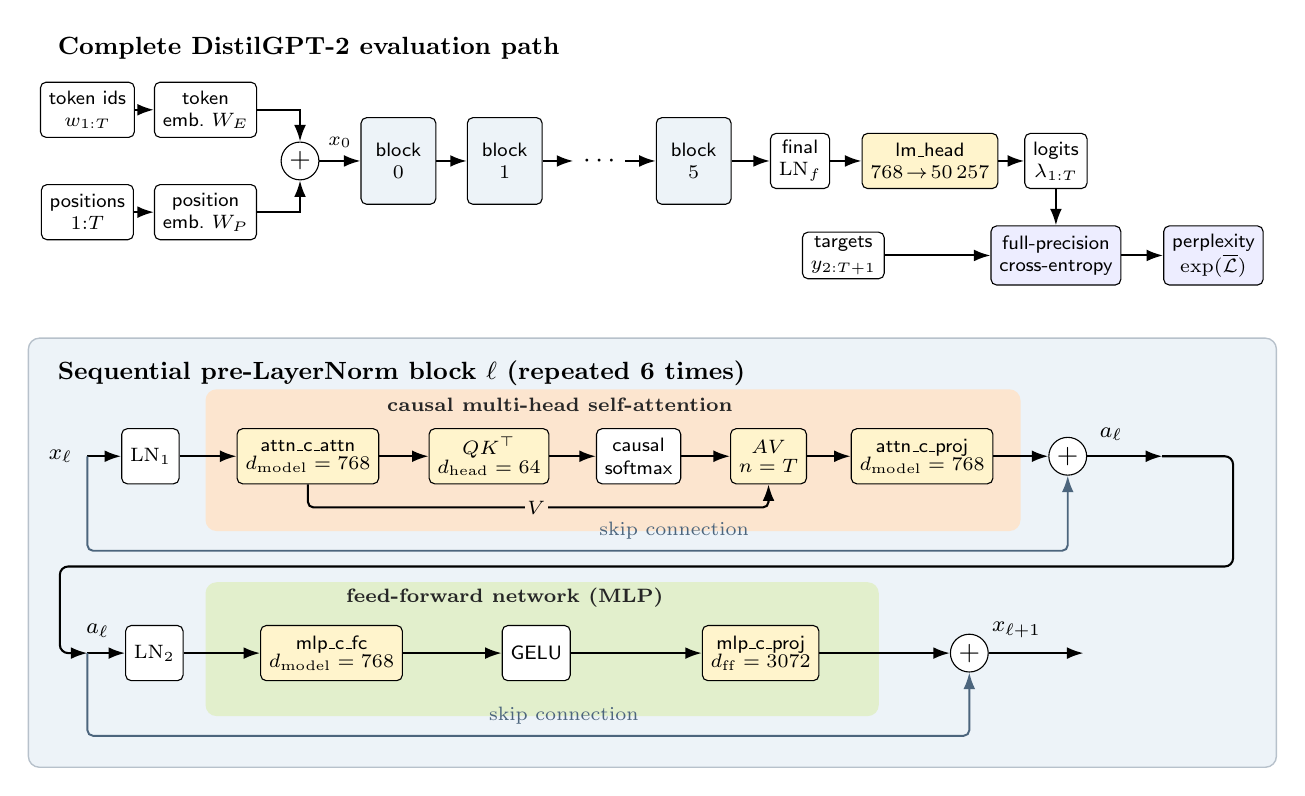
\begin{tikzpicture}[
      x=1cm,
      y=1cm,
      font=\sffamily\footnotesize,
      >={Latex[length=2.1mm,width=1.5mm]},
      flow/.style={->,line width=0.75pt},
      residual/.style={->,line width=0.7pt,draw=gptresidual},
      tie/.style={<->,densely dashed,line width=0.65pt,draw=gptresidual},
      operation/.style={
          draw,
          rounded corners=2pt,
          fill=white,
          minimum height=7mm,
          inner xsep=3pt,
          inner ysep=1.5pt,
          align=center,
          font=\sffamily\scriptsize
        },
      reduction/.style={operation,fill=gptreduction},
      block/.style={operation,fill=gptpanel,minimum width=9.5mm,minimum height=11mm},
      metric/.style={operation,fill=blue!7,minimum height=7.5mm},
      add/.style={
          circle,
          draw,
          fill=white,
          minimum size=4.8mm,
          inner sep=0pt,
          font=\normalsize
        }
      ]

% ==================================================================
      % TOP PANEL: Complete DistilGPT-2 evaluation path (no background)
      % ==================================================================
      \node[anchor=north west,font=\bfseries\small]
      at (0.05, 8.05) {Complete DistilGPT-2 evaluation path};

      % Input embeddings
      \node[operation] (tokens) at (0.55, 7.00) {token ids\\$w_{1:T}$};
      \node[operation] (positions) at (0.55, 5.70) {positions\\$1{:}T$};
      \node[operation] (wte) at (2.05, 7.00) {token\\emb.\ $W_E$};
      \node[operation] (wpe) at (2.05, 5.70) {position\\emb.\ $W_P$};
      \node[add] (embadd) at (3.25, 6.35) {$+$};

      % Transformer blocks stack (highlighted with gptpanel blue fill)
      \node[block] (bzero) at (4.50, 6.35) {block\\$0$};
      \node[block] (bone) at (5.85, 6.35) {block\\$1$};
      \node[draw=none,font=\bfseries] (dots) at (7.05, 6.35) {$\cdots$};
      \node[block] (bfive) at (8.25, 6.35) {block\\$5$};

      % Head & Logits
      \node[operation] (lnf) at (9.60, 6.35) {final\\$\mathrm{LN}_f$};
      \node[reduction] (head) at (11.25, 6.35) {\code{lm\_head}\\$768\!\to\!50\,257$};
      \node[operation] (logits) at (12.85, 6.35) {logits\\$\lambda_{1:T}$};

      % Evaluation metrics
      \node[operation,minimum height=5.5mm] (targets) at (10.15, 5.15) {targets\\$y_{2:T+1}$};
      \node[metric] (loss) at (12.85, 5.15) {full-precision\\cross-entropy};
      \node[metric] (ppl) at (14.85, 5.15) {perplexity\\$\exp(\overline{\mathcal L})$};

      % Connections in top panel
      \draw[flow] (tokens) -- (wte);
      \draw[flow] (positions) -- (wpe);
      \draw[flow] (wte.east) -| (embadd.north);
      \draw[flow] (wpe.east) -| (embadd.south);

      \draw[flow] (embadd) -- node[above=1pt,font=\scriptsize] {$x_0$} (bzero);
      \draw[flow] (bzero) -- (bone);
      \draw[flow] (bone) -- (dots);
      \draw[flow] (dots) -- (bfive);
      \draw[flow] (bfive) -- (lnf);
      \draw[flow] (lnf) -- (head);
      \draw[flow] (head) -- (logits);

      % Metrics connections
      \draw[flow] (logits) -- (loss);
      \draw[flow] (targets) -- (loss);
      \draw[flow] (loss) -- (ppl);


      % ==================================================================
      % BOTTOM PANEL: One sequential pre-LayerNorm block (zoomed, gptpanel blue)
      % ==================================================================
      \fill[gptpanel,rounded corners=4pt,draw=gptresidual!40,line width=0.5pt]
      (-0.20, -1.35) rectangle (15.65, 4.10);

      \node[anchor=north west,font=\bfseries\small]
      at (0.05, 3.93) {Sequential pre-LayerNorm block $\ell$ (repeated 6 times)};

      % --- Attention sublayer ---
      \fill[gptattention,rounded corners=4pt]
      (2.05, 1.65) rectangle (12.40, 3.45);
      \node[font=\bfseries\scriptsize,text=black!85]
      at (6.55, 3.25) {causal multi-head self-attention};

      \coordinate (xin) at (0.55, 2.60);
      \node[anchor=east] at (0.48, 2.60) {$x_\ell$};
      \node[operation] (lnone) at (1.35, 2.60) {$\mathrm{LN}_1$};
      \node[reduction] (cattn) at (3.35, 2.60)
      {\code{attn\_c\_attn}\\[-0.45mm]$d_{\rm model}=768$};
      \node[reduction] (qk) at (5.65, 2.60)
      {$QK^\top$\\[-0.45mm]$d_{\rm head}=64$};
      \node[operation] (softmax) at (7.55, 2.60)
      {causal\\softmax};
      \node[reduction] (av) at (9.20, 2.60)
      {$AV$\\[-0.45mm]$n=T$};
      \node[reduction] (attnproj) at (11.15, 2.60)
      {\code{attn\_c\_proj}\\[-0.45mm]$d_{\rm model}=768$};
      \node[add] (addone) at (13.00, 2.60) {$+$};
      \coordinate (amid) at (14.20, 2.60);
      \node[anchor=south] at (13.55, 2.67) {$a_\ell$};

      \draw[flow] (xin) -- (lnone.west);
      \draw[flow] (lnone.east) -- (cattn.west);
      \draw[flow] (cattn.east) -- (qk.west);
      \draw[flow] (qk.east) -- (softmax.west);
      \draw[flow] (softmax.east) -- (av.west);
      \draw[flow,rounded corners=2pt]
      (cattn.south) -- (3.35, 1.95) -- (9.20, 1.95) -- (av.south);
      \node[font=\scriptsize,fill=gptattention,inner sep=1pt]
      at (6.25, 1.95) {$V$};
      \draw[flow] (av.east) -- (attnproj.west);
      \draw[flow] (attnproj.east) -- (addone.west);
      \draw[flow] (addone.east) -- (amid);

      % Attention skip connection (below the orange box)
      \draw[residual,rounded corners=2pt]
      (xin) -- (0.55, 1.40) -- (13.00, 1.40) -- (addone.south);
      \node[anchor=south,draw=none,font=\scriptsize,text=gptresidual]
      at (8.00, 1.42) {skip connection};

      % --- MLP sublayer ---
      \fill[gptmlp,rounded corners=4pt]
      (2.05, -0.70) rectangle (10.60, 1.00);
      \node[font=\bfseries\scriptsize,text=black!85]
      at (5.85, 0.80) {feed-forward network (MLP)};

      \coordinate (ain) at (0.55, 0.10);
      \node[anchor=south] at (0.68, 0.18) {$a_\ell$};
      \node[operation] (lntwo) at (1.40, 0.10) {$\mathrm{LN}_2$};
      \node[reduction] (fc) at (3.65, 0.10)
      {\code{mlp\_c\_fc}\\[-0.45mm]$d_{\rm model}=768$};
      \node[operation,fill=white] (gelu) at (6.25, 0.10) {GELU};
      \node[reduction] (mlpproj) at (9.10, 0.10)
      {\code{mlp\_c\_proj}\\[-0.45mm]$d_{\rm ff}=3072$};
      \node[add] (addtwo) at (11.75, 0.10) {$+$};
      \coordinate (xout) at (13.20, 0.10);
      \node[anchor=south] at (12.35, 0.17) {$x_{\ell+1}$};

      \draw[flow] (ain) -- (lntwo.west);
      \draw[flow] (lntwo.east) -- (fc.west);
      \draw[flow] (fc.east) -- (gelu.west);
      \draw[flow] (gelu.east) -- (mlpproj.west);
      \draw[flow] (mlpproj.east) -- (addtwo.west);
      \draw[flow] (addtwo.east) -- (xout);

      % MLP skip connection
      \draw[residual,rounded corners=2pt]
      (ain) -- (0.55, -0.95) -- (11.75, -0.95) -- (addtwo.south);
      \node[anchor=south,draw=none,font=\scriptsize,text=gptresidual]
      at (6.60, -0.93) {skip connection};

      % Sublayer-to-sublayer transition arrow (amid -> ain)
      \draw[flow,rounded corners=3pt]
      (amid) -- (15.10, 2.60) -- (15.10, 1.20) --
      (0.20, 1.20) -- (0.20, 0.10) -- (ain);

        \end{tikzpicture}%
  }
  \caption{Complete DistilGPT-2 architecture and evaluation path. Token and
    position embeddings form $x_0$, which passes sequentially through six
    pre-LayerNorm GPT-2 blocks. The lower panel expands the
    repeated block into its attention and MLP sublayers. Yellow nodes identify the groups
    instrumented by the rounding experiments.}
  \label{fig:architecture}
\end{figure}

